% =====================================================================
% RoadVision — IEEE conference-format project report (19MAM56 AML Lab, CAT II)
% Compile on Overleaf (IEEEtran is built in) or locally: pdflatex x2.
% All numbers come from report/tables/*.tex, generated by
%   python scripts/run_pipeline.py --stages report
% Lines marked  %% EDIT-AFTER-RUN  hold interpretation you should re-read once
% your real results are in.
% =====================================================================
\IfFileExists{IEEEtran.cls}{\documentclass[conference]{IEEEtran}}%
  {\documentclass[10pt,twocolumn,a4paper]{article}% Used only when IEEEtran.cls is not installed (Overleaf has it; this lets plain TeX Live compile a close look-alike).
\usepackage[margin=0.7in,columnsep=0.25in]{geometry}
\usepackage{times}
\newcommand{\IEEEauthorblockN}[1]{#1\\}
\newcommand{\IEEEauthorblockA}[1]{\small #1}
\newenvironment{IEEEkeywords}{\par\noindent\textbf{\textit{Index Terms}---}\itshape}{\par}
}
\usepackage{amsmath,amssymb,amsfonts}
\usepackage{graphicx,booktabs,multirow,xcolor,url}
\usepackage[hidelinks]{hyperref}
\usepackage{tikz}
\usetikzlibrary{positioning,arrows.meta,fit,backgrounds}

% ---------- result macros (overwritten by tables/macros.tex) ----------
\providecommand{\NImages}{--}\providecommand{\NBoxes}{--}\providecommand{\NTrain}{--}
\providecommand{\NVal}{--}\providecommand{\NTest}{--}\providecommand{\HybF}{--}
\providecommand{\HybMAP}{--}\providecommand{\HybFPS}{--}\providecommand{\YoloF}{--}
\providecommand{\YoloFPS}{--}\providecommand{\DeltaF}{--}\providecommand{\DeltaCI}{--}
\providecommand{\PVal}{--}\providecommand{\Alpha}{--}\providecommand{\FPbg}{--}\providecommand{\FPcls}{--}
\IfFileExists{tables/macros.tex}{\renewcommand{\NImages}{2,378}
\renewcommand{\NBoxes}{4,296}
\renewcommand{\NTrain}{1,902}
\renewcommand{\NVal}{237}
\renewcommand{\NTest}{239}
\renewcommand{\HybF}{0.644}
\renewcommand{\HybMAP}{0.609}
\renewcommand{\HybFPS}{23.4}
\renewcommand{\Alpha}{0.70}
\renewcommand{\YoloF}{0.638}
\renewcommand{\YoloFPS}{48.8}
\renewcommand{\DeltaF}{+0.006}
\renewcommand{\DeltaCI}{[-0.009, 0.021]}
\renewcommand{\PVal}{0.227}
\renewcommand{\FPbg}{35\%}
\renewcommand{\FPcls}{7\%}
}{}

\newcommand{\fig}[2]{\IfFileExists{figures/#1.png}{\includegraphics[width=#2]{figures/#1.png}}%
  {\fbox{\parbox[c][2.2cm][c]{\dimexpr#2-2\fboxsep-2\fboxrule\relax}{\centering\scriptsize\texttt{\detokenize{#1}.png}\\ generated by the pipeline}}}}
\newcommand{\tab}[1]{\IfFileExists{tables/#1.tex}{\input{tables/#1.tex}}{\begin{table}[t]\centering\fbox{\scriptsize table \texttt{\detokenize{#1}} -- run the pipeline}\end{table}}}

\begin{document}
\title{RoadVision: Real-Time Road Damage Detection using YOLO and Vision Transformers}

\author{\IEEEauthorblockN{DAKSHINESH S}
\IEEEauthorblockA{M.Sc.\ Artificial Intelligence \& Machine Learning (III Year, Sem.\ V)\\
Department of Computing -- AI \& ML, Coimbatore Institute of Technology, Coimbatore -- 641014, India\\
19MAM56 Advanced Machine Learning Lab -- CAT II Project}}

\maketitle

% =====================================================================
\begin{abstract}
Manual road inspection is slow, subjective and expensive, while cracks and potholes grow quickly once water enters the pavement. We present \emph{RoadVision}, an end-to-end system that detects four damage classes---longitudinal (D00), transverse (D10) and alligator (D20) cracks and potholes (D40)---in smartphone and dash-camera images of the multi-national RDD2022 dataset. The method is a two-stage cascade: a YOLO detector proposes candidate regions in real time, and a Vision Transformer (ViT) fine-tuned on context-padded crops, including a background class built by hard-negative mining, re-labels and re-scores each proposal. A fusion weight $\alpha$ and all decision thresholds are calibrated on the validation split only. Hyper-parameters are optimised with Bayesian search (Optuna TPE) and every run is tracked in MLflow. Under the CRDDC'2022 protocol (IoU$>$0.5, matching label) the hybrid achieves F1 = \HybF{} (mAP50 \HybMAP{}) at \HybFPS{} FPS, against \YoloF{} for YOLO alone (paired bootstrap $\Delta$F1 = \DeltaF{}, 95\% CI \DeltaCI{}). %% EDIT-AFTER-RUN
We benchmark against an RT-DETR transformer detector, a weighted-boxes-fusion ensemble and published challenge and journal results, report error taxonomy, size and country breakdowns, attention-rollout and Eigen-CAM explanations, and deploy the model as a validated FastAPI service with a Gradio UI in a Docker container on Hugging Face Spaces.
\end{abstract}

\begin{IEEEkeywords}
road damage detection, YOLO, vision transformer, RT-DETR, RDD2022, hyper-parameter optimisation, explainable AI, MLOps
\end{IEEEkeywords}

% =====================================================================
\section{Introduction}
Road surface distress is the leading driver of road maintenance cost and a direct safety hazard for two-wheelers, which dominate Indian traffic. Visual surveys by engineers cover only a fraction of the network and are subjective. Because almost every vehicle now carries a camera, automatic damage detection from crowd-sensed images can turn every trip into a road survey~\cite{maeda2018,arya2021}.

The problem is hard for an object detector: cracks are thin, elongated and low-contrast; crack subtypes differ by orientation and topology rather than texture; shadows, lane markings, manhole covers and repaired patches look like damage; and image statistics shift across countries and capture devices~\cite{rdd2022}. Challenge winners address this with large ensembles that are too slow for edge deployment~\cite{crddc2022,grddc2020}.

\textbf{Objectives.} (i) Build a reproducible data-engineering pipeline for RDD2022 with auditable cleaning, stratified splitting and augmentation; (ii) design a real-time detector that combines the speed of YOLO with the global context modelling of Vision Transformers; (iii) tune it automatically with Bayesian optimisation and track every experiment; (iv) benchmark against transformer detectors, ensembles and published state of the art with statistical rigour and error analysis; and (v) deploy it as a validated API and public web application.

\textbf{Contributions.} (1) A YOLO$\rightarrow$ViT cascade with an explicit background class learned from mined false positives, and a two-parameter fusion rule calibrated on validation data; (2) a single evaluation harness that scores all models under the CRDDC protocol with bootstrap confidence intervals and a paired significance test; (3) a fully containerised deployment with input validation and a maintenance-priority severity index.

% =====================================================================
\section{Literature Review}
\textbf{Datasets and challenges.} Maeda \emph{et al.}~\cite{maeda2018} released the first large smartphone road-damage dataset (Japan) and trained SSD detectors. It grew into RDD2020 (Japan, India, Czech Republic) for the IEEE BigData Global Road Damage Detection Challenge, whose winning YOLO ensemble reached F1 $\approx$ 0.67 / 0.66 on the two test sets~\cite{grddc2020,arya2021}. RDD2022 adds Norway, the USA and China (47{,}420 images, six countries)~\cite{rdd2022}. In CRDDC'2022 the best overall F1 was 0.770, obtained by an ensemble of YOLOv5/YOLOv7 with a Cascade R-CNN~\cite{cascade} using a Swin Transformer backbone~\cite{swin}; the best single model (YOLOv7, third place) scored 0.741~\cite{crddc2022}. Country-level F1 varied from 0.58 (India) to 0.84 (USA) for the same winning model, showing strong domain shift.

\textbf{Detectors.} One-stage YOLO detectors~\cite{yolo,yolov8} dominate the leaderboards because of their speed--accuracy trade-off. Two-stage detectors such as Faster R-CNN~\cite{fasterrcnn} are more accurate on small objects but slower. DETR~\cite{detr} removed hand-crafted anchors and NMS through set prediction, and RT-DETR~\cite{rtdetr} made transformer detection real-time.

\textbf{Vision Transformers.} ViT~\cite{vit} models an image as a sequence of patches with global self-attention, which suits long, thin structures that span many receptive fields; with ImageNet-21k pre-training and strong augmentation it transfers well to small datasets~\cite{steiner}.

\textbf{Recent work.} StripRFNet~\cite{striprfnet} (2025) adds strip receptive fields and shape-aware modules to a YOLO-style network and reports F1 = 0.816 on the Chinese subset of RDD2022, against 0.807 for YOLOv8s and 0.767 for RT-DETRv2-R18 under a random 8:1:1 split.

\textbf{Research gaps.} (G1) Leading results depend on heavy multi-model ensembles that are impractical in real time; (G2) most errors are confusions between crack subtypes and background false alarms, yet few works add a dedicated verification stage; (G3) results are rarely reported with confidence intervals, error taxonomies or explanations; (G4) few studies ship a deployable, validated system. RoadVision addresses G1--G4.

% =====================================================================
\section{Methodology}
\subsection{System overview}
Fig.~\ref{fig:block} shows the pipeline. Raw VOC annotations are cleaned and split, YOLO and RT-DETR are trained on full images, a ViT is trained on crops, and the cascade is calibrated on validation data before a single test evaluation.

\begin{figure*}[t]\centering
\resizebox{\textwidth}{!}{%
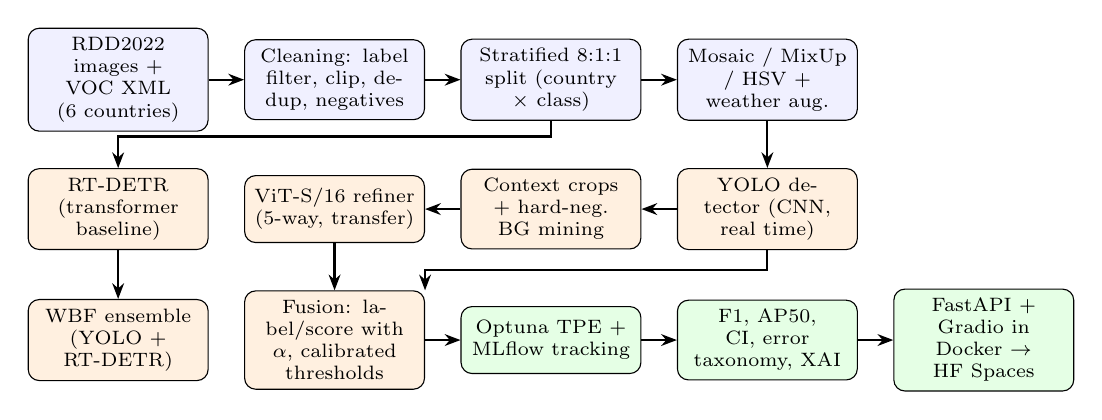
\begin{tikzpicture}[node distance=0.35cm and 0.45cm, every node/.style={font=\scriptsize},
  b/.style={draw,rounded corners,fill=blue!6,align=center,minimum height=0.85cm,text width=2.05cm},
  m/.style={draw,rounded corners,fill=orange!12,align=center,minimum height=0.85cm,text width=2.05cm},
  d/.style={draw,rounded corners,fill=green!10,align=center,minimum height=0.85cm,text width=2.05cm},
  a/.style={-{Stealth[length=2mm]},thick}]
\node[b] (raw) {RDD2022 images + VOC XML (6 countries)};
\node[b,right=of raw] (clean) {Cleaning: label filter, clip, de-dup, negatives};
\node[b,right=of clean] (split) {Stratified 8:1:1 split (country $\times$ class)};
\node[b,right=of split] (aug) {Mosaic / MixUp / HSV + weather aug.};
\node[m,below=0.6cm of aug] (yolo) {YOLO detector (CNN, real time)};
\node[m,left=of yolo] (crops) {Context crops + hard-neg.\ BG mining};
\node[m,left=of crops] (vit) {ViT-S/16 refiner (5-way, transfer)};
\node[m,left=of vit] (rt) {RT-DETR (transformer baseline)};
\node[m,below=0.6cm of vit] (fuse) {Fusion: label/score with $\alpha$, calibrated thresholds};
\node[m,left=of fuse] (wbf) {WBF ensemble (YOLO + RT-DETR)};
\node[d,right=of fuse] (opt) {Optuna TPE + MLflow tracking};
\node[d,right=of opt] (eval) {F1, AP50, CI, error taxonomy, XAI};
\node[d,right=of eval] (dep) {FastAPI + Gradio in Docker $\rightarrow$ HF Spaces};
\draw[a] (raw)--(clean); \draw[a] (clean)--(split); \draw[a] (split)--(aug); \draw[a] (aug)--(yolo);
\draw[a] (yolo)--(crops); \draw[a] (crops)--(vit); \draw[a] (vit)--(fuse); \draw[a] (yolo.south) |- ++(0,-0.25) -| (fuse.north east);
\draw[a] (split.south) |- ++(0,-0.2) -| (rt.north); \draw[a] (rt)--(wbf); \draw[a] (fuse)--(opt); \draw[a] (opt)--(eval); \draw[a] (eval)--(dep);
\end{tikzpicture}}
\caption{RoadVision block diagram: data engineering (blue), modelling (orange), optimisation, evaluation and deployment (green).}\label{fig:block}
\end{figure*}

\subsection{Data preprocessing pipeline}
RDD2022 annotations are Pascal-VOC XML. We keep the four challenge classes and drop rare or out-of-scope labels (D43, D44, D50, Repair). Boxes are clipped to the image, boxes thinner than 4\,px are removed as annotation noise, and exact duplicates are removed. Images without any damage (a form of missing labels) are not discarded but sub-sampled to 15\% of the labelled count and kept as hard negatives. Corrupt images or XML files are skipped. Every step is counted (Table~\ref{tab:clean}). After cleaning, \NImages{} images with \NBoxes{} boxes remain. Norway (3650$\times$2044\,px, 9.9\,GB) is excluded from the default run to fit a single 16\,GB GPU.

The split is stratified on the joint key \emph{country}$\times$\emph{dominant class}, so every country and class appears in train (\NTrain{}), validation (\NVal{}) and test (\NTest{}). Rare strata are merged into their country. Training uses Ultralytics mosaic, MixUp, HSV and geometric augmentation for the detectors, and an Albumentations~\cite{albu} pipeline that simulates dash-cam conditions (motion blur, rain, fog, shadows, CLAHE) for the ViT.

\tab{cleaning}

\subsection{Stage 1 -- YOLO detector}
YOLO (v8/11) predicts per anchor-free grid cell a box and class scores. Its loss is
\begin{equation}
\mathcal{L}_{\text{YOLO}} = \lambda_{\text{box}}\,\mathcal{L}_{\text{CIoU}} + \lambda_{\text{cls}}\,\mathcal{L}_{\text{BCE}} + \lambda_{\text{dfl}}\,\mathcal{L}_{\text{DFL}},
\end{equation}
where CIoU penalises overlap, centre distance and aspect-ratio mismatch, and the distribution focal loss (DFL) refines box edges. At inference we keep proposals with confidence $\geq 0.05$ after NMS, deliberately favouring recall, because the ViT will remove false positives.

\subsection{Stage 2 -- Vision Transformer refiner}
Each proposal $b$ is enlarged by 15\% context and resized to $224{\times}224$, then split into $N{=}196$ patches $x_p^i\in\mathbb{R}^{16\cdot16\cdot3}$:
\begin{align}
z_0 &= [x_{\text{cls}};\,x_p^1E;\dots;x_p^NE] + E_{\text{pos}},\\
z'_\ell &= \mathrm{MSA}(\mathrm{LN}(z_{\ell-1})) + z_{\ell-1},\quad z_\ell = \mathrm{MLP}(\mathrm{LN}(z'_\ell)) + z'_\ell,\\
\mathrm{Attn}(Q,K,V) &= \mathrm{softmax}\!\left(QK^{\top}/\sqrt{d_k}\right)V .
\end{align}
The class token $z_L^0$ is mapped to $K{+}1{=}5$ logits (D00, D10, D20, D40, BG). The BG class is trained on random road patches and on \emph{hard negatives}: YOLO detections on the training split that match no ground truth (IoU$<$0.3). We fine-tune an ImageNet-21k ViT-S/16~\cite{vit,timm} with AdamW, a lower backbone learning rate (differential transfer learning), cosine schedule with warm-up, stochastic depth, label smoothing~\cite{szegedy} and a class-balanced sampler:
\begin{equation}
\mathcal{L}_{\text{ViT}} = -\sum_{k=1}^{K+1}\big[(1-\varepsilon)\,y_k + \tfrac{\varepsilon}{K+1}\big]\log p_k .
\end{equation}

\subsection{Cascade fusion}
For a proposal with YOLO label $c_y$, confidence $s_y$ and ViT posterior $p$, let $\tilde p_k = p_k/\sum_{j\le K}p_j$ and $p_{\text{bg}}=p_{K+1}$. Then
\begin{align}
\hat c &= \arg\max_k\;\alpha\,\mathbb{1}[k=c_y] + (1-\alpha)\,\tilde p_k,\\
\hat s &= s_y^{\,\alpha}\,\big[(1-p_{\text{bg}})\,\tilde p_{\hat c}\big]^{1-\alpha}.
\end{align}
$\alpha{=}1$ recovers YOLO, $\alpha{=}0$ trusts only the ViT. $\alpha\in\{0,0.1,\dots,1\}$ and the score threshold are chosen by grid search to maximise validation F1 (selected $\alpha$ = \Alpha{}).

\subsection{Transformer detector and ensemble baselines}
RT-DETR~\cite{rtdetr} (ResNet/HGNet backbone, hybrid encoder, IoU-aware query selection) is trained with the Hungarian set-prediction loss $\mathcal{L}=\sum_i[\mathcal{L}_{\text{cls}}+\lambda_1\|b_i-\hat b_{\sigma(i)}\|_1+\lambda_2\mathcal{L}_{\text{GIoU}}]$. We also fuse YOLO and RT-DETR outputs with Weighted Boxes Fusion~\cite{wbf}, which averages the coordinates of overlapping boxes weighted by confidence$\times$model weight and penalises boxes that only one model predicts.

\subsection{Hyper-parameter search strategy}
We use Optuna~\cite{optuna} with the multivariate Tree-structured Parzen Estimator~\cite{tpe}, which models $\ell(x)=p(x\,|\,y{>}y^*)$ and $g(x)=p(x\,|\,y{\le}y^*)$ and proposes the $x$ that maximises $\ell(x)/g(x)$ (equivalent to maximising expected improvement). A median pruner stops trials whose intermediate score falls below the median of earlier trials at the same epoch. YOLO search space: $lr_0$ (log, $10^{-4}$--$2{\times}10^{-2}$), momentum, weight decay, optimiser \{SGD, AdamW\}, mosaic, MixUp, HSV value gain, rotation, box and class loss gains; objective is validation mAP50 after 15 epochs on 35\% of the training data. ViT space: learning rate, backbone LR multiplier, weight decay, label smoothing and drop-path; objective is validation macro-F1. Studies are stored in SQLite (resumable), and every trial is a nested MLflow~\cite{mlflow} run with parameters, per-epoch metrics and artefacts.

\subsection{Evaluation protocol}
Following CRDDC'2022~\cite{crddc2022}, a prediction is a true positive iff IoU$>$0.5 with an unmatched ground-truth box of the same class (greedy matching by score), and we report $F1=2PR/(P+R)$. We also report VOC all-point AP50 per class and mAP50. The threshold for each model is chosen on validation and applied unchanged to test. 95\% confidence intervals use 1{,}000 image-level bootstrap resamples~\cite{efron}; the paired test resamples the same images for both models.

% =====================================================================
\section{Implementation and Experiments}
\textbf{Environment.} Python 3.12, PyTorch 2.6 (CUDA 12.4), Ultralytics 8.4, timm 1.0, Optuna 5.0, MLflow 3.17, scikit-learn, Albumentations; training on a single NVIDIA GeForce RTX 4060 Laptop GPU (8\,GB). YOLOv8s trains at about 30\,s per epoch on this hardware.
Seeds are fixed (42) and deterministic cuDNN is enabled.

\textbf{Code organisation.} The repository is a Python package (\texttt{src/roadvision}) with sub-modules \texttt{data}, \texttt{models}, \texttt{tuning}, \texttt{evaluation}, \texttt{explain}, \texttt{visualization} and \texttt{inference}; all settings live in YAML (\texttt{configs/}); \texttt{scripts/run\_pipeline.py} executes the idempotent stages download $\rightarrow$ prepare $\rightarrow$ tune $\rightarrow$ train $\rightarrow$ evaluate $\rightarrow$ benchmark $\rightarrow$ explain $\rightarrow$ plots $\rightarrow$ report. Unit tests cover data conversion, metrics and the API contract.

\textbf{Training settings (reduced-budget run).} This is a fast-track, reduced-budget experiment on the RDD2022 China subset (China\_MotorBike + China\_Drone) with the \texttt{china\_811} protocol (random 8:1:1 split). Because the official CRDDC bucket was unreachable, data came from the public Hugging Face mirror \texttt{dronefreak/RDD2022} (4-class export), which retains 2{,}378 of the China images (1{,}902/237/239 train/val/test, 4{,}296 boxes); results are therefore only approximately comparable with StripRFNet~\cite{striprfnet}, which used the full China subset. YOLOv8s, 512\,px, 15 epochs, batch 32, cosine LR, mosaic closed for the final 3 epochs, default hyper-parameters (the YOLO Optuna search was skipped for time). ViT-S/16 (ImageNet-21k), 4 epochs, batch 64, with a 3-trial Optuna TPE search (1 epoch per trial). RT-DETR and the WBF ensemble were not trained in this run.

\textbf{Exploratory analysis.} Fig.~\ref{fig:eda} shows strong class imbalance and country-dependent class mixes (domain shift), and that most boxes cover less than 1\% of the image and are either very wide (transverse) or very tall (longitudinal). Box centres concentrate in the lower half of the frame (the road surface).

\begin{figure}[t]\centering
\fig{01_class_distribution}{\columnwidth}\\[2pt]
\fig{02_box_geometry}{\columnwidth}
\caption{Class distribution by country (top) and box geometry: relative area, aspect ratio and centre heat-map (bottom).}\label{fig:eda}
\end{figure}

\textbf{Training behaviour and tuning.} Fig.~\ref{fig:train} plots the loss and validation metrics; Fig.~\ref{fig:optuna} shows the Optuna optimisation history and parameter importance.

\begin{figure}[t]\centering
\fig{04_detector_training_curves}{\columnwidth}\\[2pt]
\fig{05_vit_training_curves}{0.85\columnwidth}
\caption{Detector training curves (top) and ViT refiner curves (bottom).}\label{fig:train}
\end{figure}

\begin{figure}[t]\centering
\fig{16_optuna_history_yolo}{0.49\columnwidth}\hfill\fig{17_optuna_importance_yolo}{0.49\columnwidth}
\caption{Optuna TPE search for YOLO: optimisation history and fANOVA hyper-parameter importance.}\label{fig:optuna}
\end{figure}

\textbf{Representation and explainability.} Fig.~\ref{fig:emb} projects ViT class-token embeddings of validation/test crops with PCA, t-SNE~\cite{tsne} and UMAP~\cite{umap}. Well separated clusters indicate that the refiner has learnt discriminative features; overlap between D00 and D10 shows where confusion remains. Attention rollout~\cite{rollout} (Fig.~\ref{fig:xai}, top) shows the ViT attending along the crack path rather than to lane paint. Eigen-CAM~\cite{eigencam} on the YOLO neck (bottom) confirms that detector activations sit on the damage. %% EDIT-AFTER-RUN

\begin{figure*}[t]\centering
\fig{13_vit_embeddings}{0.95\textwidth}
\caption{ViT embedding space: PCA cumulative variance and 2-D PCA, t-SNE and UMAP projections coloured by class.}\label{fig:emb}
\end{figure*}

\begin{figure}[t]\centering
\fig{14_vit_attention_rollout}{\columnwidth}\\[2pt]
\fig{15_yolo_eigencam}{\columnwidth}
\caption{Explainability: ViT attention rollout on test crops (top) and YOLO Eigen-CAM (bottom).}\label{fig:xai}
\end{figure}

% =====================================================================
\section{Results and Comparative Analysis}
\tab{main_results}
\tab{per_class}

\textbf{Main results.} Table~\ref{tab:main} compares all models on the held-out test split. The hybrid cascade reaches F1 = \HybF{} versus \YoloF{} for YOLO alone. The paired bootstrap gives $\Delta$F1 = \DeltaF{} (95\% CI \DeltaCI{}, one-sided $p$ = \PVal{}); a CI that excludes zero indicates a statistically reliable gain. The ViT costs extra time per proposal, so throughput falls from \YoloFPS{} to \HybFPS{} FPS, still real-time for dash-cam video sampled at a few frames per second. %% EDIT-AFTER-RUN
Per-class AP50 (Table~\ref{tab:perclass}, Fig.~\ref{fig:pr}) shows which damage types benefit most from global attention.

\begin{figure*}[t]\centering
\fig{07_pr_curves}{0.95\textwidth}
\caption{Per-class precision--recall curves on the test split for all models.}\label{fig:pr}
\end{figure*}

\textbf{Ablation.} Table~\ref{tab:ablation} isolates the cascade components. Removing the background class (setting $p_{\text{bg}}{=}0$) measures the value of hard-negative mining; $\alpha{=}0$ and $\alpha{=}1$ give the ViT-only and YOLO-only extremes. Fig.~\ref{fig:cal} shows the validation F1 as a function of $\alpha$ and of the confidence threshold.
\tab{ablation}

\begin{figure}[t]\centering
\fig{09_alpha_calibration}{0.49\columnwidth}\hfill\fig{08_f1_threshold_curves}{0.49\columnwidth}
\caption{Validation calibration: F1 vs.\ fusion weight $\alpha$ (left) and vs.\ confidence threshold (right).}\label{fig:cal}
\end{figure}

\textbf{Comparison with the state of the art.} Table~\ref{tab:bench} and Fig.~\ref{fig:bench} place RoadVision among published results. Only rows that share our protocol (RDD2022-China, random 8:1:1; run \texttt{configs/china\_811.yaml}) are directly comparable with StripRFNet~\cite{striprfnet}. Challenge results~\cite{grddc2020,crddc2022} were computed on hidden test sets whose labels are not public, so they are shown as indicative context only. %% EDIT-AFTER-RUN
\tab{benchmark}

\begin{figure}[t]\centering
\fig{12_benchmark}{\columnwidth}
\caption{F1 of RoadVision models vs.\ published detectors (colour indicates comparability).}\label{fig:bench}
\end{figure}

\textbf{Error analysis.} The confusion matrix (Fig.~\ref{fig:cm}) uses an explicit background row/column: the last column counts missed damage, the last row counts false alarms. Every hybrid false positive is assigned to one of four types (Fig.~\ref{fig:err}, left): \emph{background} (no damage nearby; \FPbg{} of FPs), \emph{classification} (right place, wrong crack type; \FPcls{}), \emph{localisation} (right class, IoU 0.1--0.5) and \emph{duplicate}. Recall by object size (right) shows that small, thin cracks remain the main source of misses, which motivates tiling or higher input resolution. Per-country F1 (Fig.~\ref{fig:country}) quantifies domain shift; the weakest country points to where more labelled data is needed. %% EDIT-AFTER-RUN

\begin{figure}[t]\centering
\fig{06_confusion_matrix}{\columnwidth}
\caption{Test confusion matrices (hybrid and YOLO); BG = background / missed.}\label{fig:cm}
\end{figure}

\begin{figure}[t]\centering
\fig{10_error_analysis}{\columnwidth}\\[2pt]
\fig{11_f1_by_country}{0.8\columnwidth}
\caption{Error taxonomy and recall by size (top); test F1 per country (bottom).}\label{fig:err}\label{fig:country}
\end{figure}

% =====================================================================
\section{Deployment}
The inference engine (\texttt{RoadVisionPredictor}) loads every available model and exposes four modes (yolo, rtdetr, hybrid, ensemble) with the calibrated thresholds. A FastAPI service provides \texttt{/predict} (JSON), \texttt{/predict/annotated} (PNG), \texttt{/predict/batch}, \texttt{/health} and \texttt{/model-info} with OpenAPI documentation. Inputs are validated by MIME type, magic bytes, a 10\,MB size limit, decodability and image-side limits; the mode is an enum and the threshold is bounded, so invalid requests return 4xx errors with explanations. Each response includes a heuristic 0--100 \emph{severity index} $S=\min\!\big(100,\tfrac{100}{1.5}\sum_i w_{c_i}\hat s_i\sqrt{A_i/A}\big)$ with weights 1/1/2/3 for D00/D10/D20/D40, mapped to Good/Fair/Poor/Critical to rank roads for maintenance. A Gradio UI is mounted at \texttt{/ui}. The same Docker image (Python 3.11-slim, CPU PyTorch, non-root user, health-check) runs locally and as a Hugging Face Docker Space; weights are pulled at start-up from a Hugging Face model repository.

% =====================================================================
\section{Conclusion and Future Scope}
RoadVision shows that a lightweight cascade---a fast CNN detector that proposes and a Vision Transformer that verifies---can address the two dominant error modes in road-damage detection, crack-type confusion and background false alarms, without the cost of a multi-model challenge ensemble. %% EDIT-AFTER-RUN
Calibrating on validation only, bootstrap confidence intervals and a fixed CRDDC-style protocol make the comparison with baselines reliable, and the containerised API makes the model usable in practice.

\textbf{Deployment considerations.} The ViT adds latency proportional to the number of proposals; batching crops, INT8/ONNX export and capping proposals keep it real-time on edge GPUs. Thresholds should be re-calibrated when the camera type or country changes, and GPS tags are needed to turn detections into maintenance maps.

\textbf{Future work.} (i) Tiled inference and higher resolution for small cracks and the Norway subset; (ii) domain adaptation across countries; (iii) instance segmentation for crack length and pothole area estimation; (iv) temporal tracking across video frames for de-duplication; (v) knowledge distillation of the ViT into the detector head for single-stage speed. Due to the lab time budget, models were trained for a reduced number of epochs on the China subset; full-dataset training is expected to improve results.

% =====================================================================
\begin{thebibliography}{99}\small
\bibitem{maeda2018} H. Maeda, Y. Sekimoto, T. Seto, T. Kashiyama, and H. Omata, ``Road damage detection and classification using deep neural networks with smartphone images,'' \emph{Computer-Aided Civil and Infrastructure Engineering}, vol.~33, no.~12, pp.~1127--1141, 2018.
\bibitem{arya2021} D. Arya, H. Maeda, S. K. Ghosh, D. Toshniwal, A. Mraz, T. Kashiyama, and Y. Sekimoto, ``Deep learning-based road damage detection and classification for multiple countries,'' \emph{Automation in Construction}, vol.~132, Art.~no.~103935, 2021.
\bibitem{grddc2020} D. Arya, H. Maeda, S. K. Ghosh, D. Toshniwal, H. Omata, T. Kashiyama, and Y. Sekimoto, ``Global road damage detection: State-of-the-art solutions,'' in \emph{Proc. IEEE Int. Conf. Big Data}, 2020. [Online]. Available: arXiv:2011.08740
\bibitem{rdd2022} D. Arya, H. Maeda, S. K. Ghosh, D. Toshniwal, and Y. Sekimoto, ``RDD2022: A multi-national image dataset for automatic road damage detection,'' arXiv:2209.08538, 2022.
\bibitem{crddc2022} D. Arya, H. Maeda, S. K. Ghosh, D. Toshniwal, H. Omata, T. Kashiyama, and Y. Sekimoto, ``Crowdsensing-based road damage detection challenge (CRDDC'2022),'' in \emph{Proc. IEEE Int. Conf. Big Data}, 2022. [Online]. Available: arXiv:2211.11362
\bibitem{striprfnet} J. Lin, Y. Qin, S. Gao, Y. Rui, J. Liu, and Y. Lv, ``StripRFNet: A strip receptive field and shape-aware network for road damage detection,'' arXiv:2510.16115, 2025.
\bibitem{yolo} J. Redmon, S. Divvala, R. Girshick, and A. Farhadi, ``You only look once: Unified, real-time object detection,'' in \emph{Proc. IEEE Conf. Comput. Vis. Pattern Recognit. (CVPR)}, 2016, pp.~779--788.
\bibitem{yolov8} G. Jocher, A. Chaurasia, and J. Qiu, ``Ultralytics YOLO,'' 2023. [Online]. Available: https://github.com/ultralytics/ultralytics
\bibitem{fasterrcnn} S. Ren, K. He, R. Girshick, and J. Sun, ``Faster R-CNN: Towards real-time object detection with region proposal networks,'' in \emph{Proc. Adv. Neural Inf. Process. Syst. (NeurIPS)}, 2015, pp.~91--99.
\bibitem{cascade} Z. Cai and N. Vasconcelos, ``Cascade R-CNN: Delving into high quality object detection,'' in \emph{Proc. CVPR}, 2018, pp.~6154--6162.
\bibitem{swin} Z. Liu \emph{et al.}, ``Swin Transformer: Hierarchical vision transformer using shifted windows,'' in \emph{Proc. IEEE/CVF Int. Conf. Comput. Vis. (ICCV)}, 2021, pp.~10012--10022.
\bibitem{detr} N. Carion, F. Massa, G. Synnaeve, N. Usunier, A. Kirillov, and S. Zagoruyko, ``End-to-end object detection with transformers,'' in \emph{Proc. Eur. Conf. Comput. Vis. (ECCV)}, 2020, pp.~213--229.
\bibitem{rtdetr} Y. Zhao \emph{et al.}, ``DETRs beat YOLOs on real-time object detection,'' in \emph{Proc. IEEE/CVF CVPR}, 2024, pp.~16965--16974.
\bibitem{vit} A. Dosovitskiy \emph{et al.}, ``An image is worth 16x16 words: Transformers for image recognition at scale,'' in \emph{Proc. Int. Conf. Learn. Represent. (ICLR)}, 2021.
\bibitem{steiner} A. Steiner, A. Kolesnikov, X. Zhai, R. Wightman, J. Uszkoreit, and L. Beyer, ``How to train your ViT? Data, augmentation, and regularization in vision transformers,'' \emph{Trans. Mach. Learn. Res.}, 2022.
\bibitem{timm} R. Wightman, ``PyTorch image models,'' 2019. [Online]. Available: https://github.com/huggingface/pytorch-image-models
\bibitem{szegedy} C. Szegedy, V. Vanhoucke, S. Ioffe, J. Shlens, and Z. Wojna, ``Rethinking the Inception architecture for computer vision,'' in \emph{Proc. CVPR}, 2016, pp.~2818--2826.
\bibitem{wbf} R. Solovyev, W. Wang, and T. Gabruseva, ``Weighted boxes fusion: Ensembling boxes from different object detection models,'' \emph{Image and Vision Computing}, vol.~107, Art.~no.~104117, 2021.
\bibitem{optuna} T. Akiba, S. Sano, T. Yanase, T. Ohta, and M. Koyama, ``Optuna: A next-generation hyperparameter optimization framework,'' in \emph{Proc. ACM SIGKDD Int. Conf. Knowl. Discov. Data Min.}, 2019, pp.~2623--2631.
\bibitem{tpe} J. Bergstra, R. Bardenet, Y. Bengio, and B. K\'egl, ``Algorithms for hyper-parameter optimization,'' in \emph{Proc. NeurIPS}, 2011, pp.~2546--2554.
\bibitem{mlflow} M. Zaharia \emph{et al.}, ``Accelerating the machine learning lifecycle with MLflow,'' \emph{IEEE Data Eng. Bull.}, vol.~41, no.~4, pp.~39--45, 2018.
\bibitem{albu} A. Buslaev, V. I. Iglovikov, E. Khvedchenya, A. Parinov, M. Druzhinin, and A. A. Kalinin, ``Albumentations: Fast and flexible image augmentations,'' \emph{Information}, vol.~11, no.~2, Art.~no.~125, 2020.
\bibitem{rollout} S. Abnar and W. Zuidema, ``Quantifying attention flow in transformers,'' in \emph{Proc. Annu. Meeting Assoc. Comput. Linguistics (ACL)}, 2020, pp.~4190--4197.
\bibitem{eigencam} M. B. Muhammad and M. Yeasin, ``Eigen-CAM: Class activation map using principal components,'' in \emph{Proc. Int. Joint Conf. Neural Netw. (IJCNN)}, 2020.
\bibitem{tsne} L. van der Maaten and G. Hinton, ``Visualizing data using t-SNE,'' \emph{J. Mach. Learn. Res.}, vol.~9, pp.~2579--2605, 2008.
\bibitem{umap} L. McInnes, J. Healy, and J. Melville, ``UMAP: Uniform manifold approximation and projection for dimension reduction,'' arXiv:1802.03426, 2018.
\bibitem{efron} B. Efron and R. J. Tibshirani, \emph{An Introduction to the Bootstrap}. New York, NY, USA: Chapman \& Hall, 1993.
\end{thebibliography}

\end{document}
